%\author{Grace Li}
%\author{Christopher Ing}
% \author{Dustin Little}
% \author{P. Lynne Howell}
% \email{howell@sickkids.ca}
% \affiliation[University of Toronto, Biochemistry]
% {Department of Biochemistry, University of Toronto, 27 King's College Circle, Toronto, Ontario, Canada M5S 1A1}
% \alsoaffiliation[Hospital for Sick Children]
% {Molecular Structure and Function, The Hospital for Sick Children, 555 University Avenue, Toronto, Ontario, Canada M5G 1X8}
% 
% \author{Mark Nitz}
% \email{nitz@chem.utoronto.ca}
% \affiliation[University of Toronto, Chemistry]
% {Department of Chemistry, University of Toronto, 80 St. George Street, Toronto, Ontario, Canada M5S 3H6}

%\author{R\'{e}gis Pom\`{e}s}
%\email{pomes@sickkids.ca}
%\phone{416 813 5686}
%\fax{416 813 5022}
%\affiliation[University of Toronto, Biochemistry]
%{Department of Biochemistry, University of Toronto, 27 King's College Circle, Toronto, Ontario, Canada M5S 1A1}
%\alsoaffiliation[Hospital for Sick Children]
%{Molecular Structure and Function, The Hospital for Sick Children, 555 University Avenue, Toronto, Ontario, Canada M5G 1X8}

\chapter[MD simulations of PgaB-glucosamine binding]{Molecular Dynamics simulations of PgaB and monosaccharides of N-acetyl-glucosamine}
% The contents of this section were adapted from an article published in the \emph{Journal of Physical Chemistry}.

\emph{Reference}: Part of this work is published in ``PgaB Contains a Carbohydrate Binding Domain Required for Modification and Export of Poly-$\beta$-1,6-N-acetyl-D-glucosamine"
\\
\\
\emph{Contributions}:
Grace Li conducted the MD simulation part of the research and wrote the section. Dustin Little conducted and interpreted the experimental results. Chris Ing parameterized a key molecule for one of the simulations. Régis Pomès, Lynne Howell, Mark Nitz provided editorial input and guidance.

\newpage

\section{Summary}
% Note that this summary was taken from a draft of the paper written by Dustin from April 5th, 2013
Bacteria embedded in a self-produced matrix of exopolymeric substance, or biofilm, are tolerant to antibiotics, protected from the environment, and isolated from the innate immune system. Production and de-N-acetylation of the exopolysaccharide poly-$\beta$-1,6-N-acetyl-D-glucosamine (PNAG) is important for biofilm formation in Escherichia coli. PgaB is essential for the partial de-N-acetylation of PNAG (dPNAG); a process required for polymer export and subsequent biofilm formation. Here we report 1.9 Å crystal structures of PgaB’s isolated C-terminal domain (PgaB-CT) and complex with glucosamine. The structure of PgaB-CT has structural difference from the previously reported PgaB42-655 structure. Characterization of PgaB-CT using tryptophan fluorescence quenching assays shows binding to PNAG oligomers with ~1-4 mM affinity. These data in combination with molecular dynamics simulations of PgaB with N-acetylglucosamine and glucosamine suggest PNAG de-N-acetylation occurs first, with subsequent binding of dPNAG to the C-terminal domain. We believe this concerted action plays a pivotal role in targeting dPNAG for export through the outer membrane porin PgaA.

\section{Introduction}
\textbf{In the second paper, experiments were performed to characterize the ability of PgaB-CT domain to bind carbohydrate substrates, which are short oligosaccharides of \pnag. The results of this study suggests a mechanism by which polymer substrates are bound and synthesized onto the protein.  Furthermore, a proposed mechanism of export is discussed.}

\textbf{commentary: From reading what Dustin has written in the current introduction, I think their experimental data is quite weak.  Their key result is:  ``We show PgaB-CT binds PNAG oligomers with low affinity (what's the range?) using tryptophan fluorescence quenching, and have determined the structure of PgaB-CT in complex with glucosamine.'' I think MD simulations will be their best leverage for the proposed mechanism of export.}

% PgaB - description of the study, motivation and what has been done thus far
PgaB is a key protein that is responsible for the transport of the functionally relevant form of the exopolysaccharride poly-$\beta$-1,6-$N$-acetylglucosamine (PNAG), which is required for biofilm formation in a variety of bacterial systems. A crystal structure of PgaB was recently solved in the laboratory of Dr. Lynne Howell. Structural and functional characterization studies have shown that PgaB is composed of two domains, an N-terminal de-N-acetylase domain, and a C-terminal domain with structural homology to glycosyl hydrolases.\cite{Little:2012dp}
% PgaB structure has been deposited in the PDB -- I did not find this June 30th 2012

Currently, it is not known whether PgaB binds polymeric GlcNac or its de-N-acetylated end products, or both. Furthermore, binding modes, and lengths of putative substrate sugar polymers of PgaB are not known. Experimental characterization of sugar-bound structures of PgaB have been impeded by the insolubility of long sugar polymer chains (eg. those longer than a pentamer), and the weak binding of short sugar polymers (eg. di- and tri-saccharides). PgaB is hypothesized to bind sugar polymers (most likely a 15-mer) across its two domains at its surface. The polymer is speculated to extend out from the catalytic binding site (N-terminal domain) onto the charged grooves of the C-terminal domain.
% Experimentally it is known that shallow binding pockets exist at the surface of the proteins. REF?

Using molecular dynamics simulations, we exploit the weak binding affinities of N-acetyl-glucosamine (GlcNac) and glucosamine monosaccharides by using a fragment-based simulation approach to predict putative binding modes and sites of GlcNac and glucosamine. This methodology has been successfully applied in our previous simulation studies to examine the binding mechanism of inositol, a carbohydrate-like amyloid inhibitor, with amyloidogenic peptides and their aggregates. To our knowledge, this is the only study thus far in literature which employs large-scale MD simulations to predict sugar-protein interactions.

% The objective of my work is to predict PNAG binding sites at the surface of PgaB using unrestrained molecular dynamics simulations in the presence of GlcNac. This methodology was used in earlier inositol studies to predict inositol binding sites on amyloid peptides and aggregates.
\textbf{The directionality of the polymer binding.  This is currently not experimentally determined.} 

\section{Material and Methods}
% Modelling details
PgaB with a loop spanning residues 613 to 619 (numbered according to the chimeric PDB structure; check with Dustin again) in the N-terminal domain modelled into the truncated crystal structure, was used in our simulations. The initial crystal structure has Ni(II) bound at its enzymatic active site. Ni(II) is tetrahedrally coordinated with surrounding residues.  The acetate ion bound near the active site, an artifact of crystallization, was removed in the simulation. Crystal waters were removed from the initial PDB structure. Histidine protonation states were assigned based on predicted pKa values using the web software PROPKA (\url{http://propka.ki.ku.dk}), and histidine hydrogen-bonding geometries in the initial crystal structure.

Protein and ions were modelled using the AMBER99 force field.\cite{Cornell:1995td} Parameters for Ni(II) was approximated using the parameters for the magnesium ion (Mg$^{2+}$). After assigning protonation states of histidines, the net charge of the protein was -10e. The final simulation system comprised of 11 sodium (Na$^{+}$) counterions, and either 45 molecules of free $\beta$-N-acetyl-glucosamine (GlcNac) or glucosamine, at a concentration of 100 mM (Figure~\ref{fig:nag}). 19533 and 19991 water molecules were present in the GlcNac and glucosamine simulations, respectively. The initial volume of the simulation box is 713.6 nm$^{3}$.  To mimic experimental conditions, 100 mM of salt was added to the aqueous solution in glucosamine simulation systems.

% Note: To generate this structure from Glycam builder, choose the beta-pyranose ring and then acetyl-glucosamine
GlcNac molecules were generated using the web-based Glycam Biomolecule Builder (\url{http://glycam.ccrc.uga.edu/ccrc/biombuilder/biomb_index.jsp}). The GLYCAM06 force field for carbohydrates\cite{Kirschner:2008ii} was used to model GlcNac and glucosamine. A PDB of glucosamine-$\textrm{NH}_{3}^{+}$ was obtained from the ZINC database.\cite{Irwin:2005kx} Energy minimization was performed using the software GAUSSIAN-09.\cite{g09} The minimized glucosamine structure was consistent with the GLYCAM force field, and new RESP-derived partial atomic charges were computed for glucosamine (a net charge of -1e) by fitting to a single HF/6-31G* molecular electrostatic potential (MEP) with a restraint weight of 0.01. MEPs were computed using the CHELPG methodology\cite{Breneman:1990ue} with the R.E.D. III software package.\cite{Dupradeau:2010bb} The partial charges were assigned so that the HCNH3 group summed to a net charge of +1.164e, and the rest of the molecule summed to a net charge of -0.164e. Aliphatic hydrogen atoms were fitted with a zero partial charge in order to be compatible with GLYCAM06.
% How to cite the web builder - Carbohydrate Builder Woods Group. (2005-XXXX) GLYCAM Web. Complex Carbohydrate Research Center, University of Georgia, Athens, GA. (http://www.glycam.com) XXXX = current year

% Note put the partial charges used for glucosamine in an appendix. Ask Chris Ing to add to this methods description.  

The TIP3P water model was used to represent the solvent. Version 4.5.5 of the GROMACS software package\cite{Pronk:2013ef,Hess:2008p5353} was used to perform unrestrained all-atom MD simulations with the stochastic dynamics algorithm using an integration timestep of 2 femtoseconds.

% Better organize below to make clear that I was using different integrators for equilibration and production dynamics.
% I still need to remind myself what rcoulomb and rlist corresponds to physically in the MD algorithm
Electrostatic interactions were calculated using Particle Mesh Ewald (PME) summation with a grid size of 0.12 nm and a Coulombic real-space cutoff of 1.1 nm. The Lennard-Jone potential was computed up to 1.2 nm using the GROMACS twin-range cutoff function with a short-range cut-off of 1.1 nm. Covalent bonds involving hydrogens were constrained using the LINCS algorithm. The simulation system was first subjected to energy minimization followed by a 1 ns equilibration in the NVT ensemble using Berendsen temperature coupling at 300 K with a coupling constant of 2.0.

A second equilibration was performed for 1 ns in the NpT ensemble with isotropic pressure coupling. Temperature and pressure for equilibration were controlled at 300 K and at 1 atm, respectively, using Berendsen thermostat and pressure coupling schemes. Production simulations were performed using the stochastic dynamics (sd) integrator and the Parrinello-Rahman barostat for pressure coupling.
% Look at /mnt/scratch_mp2/pomes/ligrace1/pgab/protein_sugar/params for fill in the blank parameters here

13 independent MD simulations were performed for each of GlcNac and glucosamine, respectively. In total, XXX $\mu$s of sampling was performed.

\subsection*{Analysis Protocol}
To compute spatial binding probability densities of GlcNac and glucosamine, frames from our simulations were first fitted to an MD equilibrated crystal structure via RMSD alignment of the protein backbone atoms. The density map corresponds to the fractional atomic occupancy of GlcNac or glucosamine molecules in a grid with a resolution of 1 angstrom, accumulated over 900,000 time frames. The Visual Molecular Dynamics (VMD) software package\cite{Humphrey:1996to} was used to calculate and graphically render the densities depicted in Figures~\ref{fig:pgab_density} and \ref{fig:pgab_binding_sites}.
% By examining the structure - does the sugars arrange into predicted binding site (s)?

\begin{figure}[htbp]
\centering
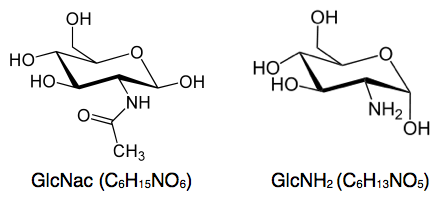
\includegraphics[height=1.5in, width=3in]{figures/results4/figure_pgab_sugars.png}
\caption[NAG]{$\beta$-N-acetyl-glucosamine (GlcNac) and glucosamine (GlcNH$_2$) monosaccharides.}
\label{fig:nag}
\end{figure}

\section{Results and Discussion}

\textbf{The spatial distribution of bound glucosamine, as depicted in Figure~\ref{fig:pnag_nag_overlapped_zoomedout}, indicates that although glucosamine molecules are able to bind on surfaces of both domains, they preferentially bind the C-terminal domain of PgaB. Specifically, clusters of glucosamine molecules are bound in the groove lined with acidic (Asp and Glu), and aromatic residues X, Y, Z (Figure~\ref{fig:nag_cterminal_zoomedin})}.  These key conserved residues are known to bind carbohydrates in other homologous carbohydrate-binding domains. \textbf{See Dustin's first pgab paper} REF In particular, our simulations suggest that glucosamine has a high affinity binding site at Trp613. Significantly, this finding is consistent with the X-ray crystal structure of full-length PgaB co-crystallized with glucosamine monosaccharides.
% This result is consistent with the homology of the C-terminal domain of PgaB to other carbohydrate binding domains. 

The spatial binding probability density of bound GlcNac, depicted in Figure~\ref{fig:pgab_density} suggests that its binding sites are localized to three main sites on PgaB (Figure~\ref{fig:pgab_binding_sites}). \textbf{There aren't 3 points here} Specifically, GlcNac predominantly binds in grooves located at the interface between the two domains, where many molecules are found to bind in clusters at the mouth of the N-terminal $\beta$-barrel, in close proximity to the active site (Figure~\ref{fig:pgab_density}).  In contrast to glucosamine, GlcNac molecules preferentially bind to residues in the N-terminal domain (Figure~\ref{fig:pgab_density}B and D).  


% When comparing the densities of PNAG and glucosamine (depicted in Figures \ref{fig:pgab_density} and XXX, respectively) it can be seen that whereas PNAG predominantly binds the N-terminal domain, but glucosamine instead bind to the C-terminal domain, predominantly in the groove capped by the loop spanning residues XXX to YYY.  

\textbf{Furthermore, in contrast to the differential binding of glucosamine and GlcNac, as depicted in Figure~\ref{fig:salt_density_distribution}, salt ions do not significant bind the protein, and are uniformly distributed over the surface of the protein.   This result further supports the ability of MD simulations and our methodology to accurately identify carbohydrate-protein recognition. Moreover, a recent study suggests that by building 3D density binding maps and combining this data with additional algorithms can increase the accuracy of identifying putative carbohydrate binding sites.\cite{Tsai:2012bj}}


\begin{figure}[htbp]
\centering
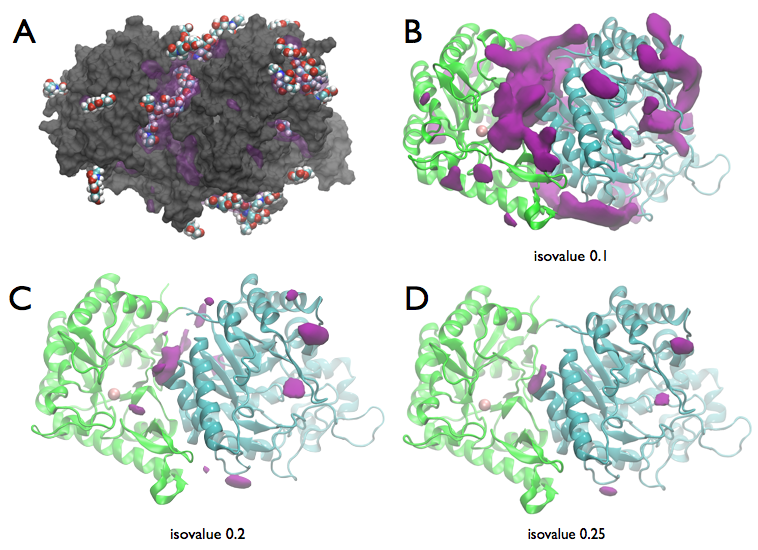
\includegraphics[height=4.25in, width=6in]{figures/results4/figure_pgab_density.png}
\caption[NAG binding density]{Spatial binding probability density map of bound GlcNac around PgaB.  (A) An example snapshot of PgaB (grey) shown using a surface representation with bound GlcNac binding density depicted in purple at 10\% occupancy (iso-contour of 0.1). Binding densities of GlcNac overlapped with a cartoon representation of PgaB at iso-contour levels of (B) 0.1 (C) 0.2 (D) 0.25. In our coloring scheme, residue numbers 43 to 310 and numbers 311 to 667 represent N- (green) and C-terminal (cyan) domains, respectively.  }
\label{fig:pgab_density}
\end{figure}

\begin{figure}[htbp]
\centering
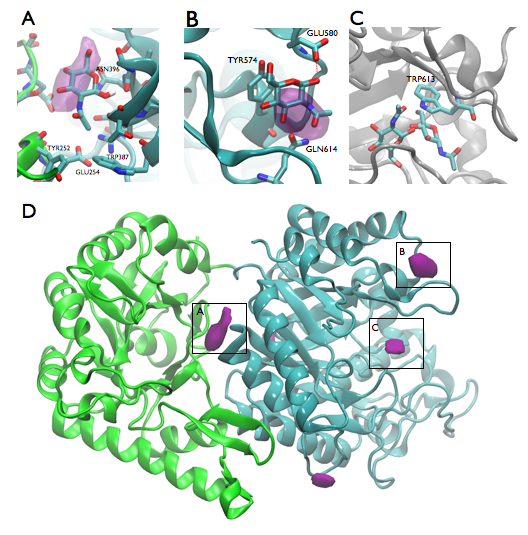
\includegraphics[height=6.29in, width=6.12in]{figures/results4/figure_pgab_binding_sites.png}
\caption[GlcNac binding sites]{High probability GlcNac binding sites at an iso-contour value of 0.25 (D). Insets (A to C) show detailed views of the binding sites and the residues involved in binding.}
\label{fig:pgab_binding_sites}
\end{figure}

% TODO: I SHOULD MAKE A NEW FIGURE HERE JUST SHOWING THE SUGAR BOUND TO THIS RESIDUE 
Both glucosamine and GlcNac were found to bind Trp 613. Notably, in our simulations, glucosamine was found to adopt a binding mode consistent with the crystal structure (Figure~\ref{fig:nag_cterminal_zoomedin}). Moreover, our simulations identified carbohydrate binding to Trp613, a key conserved residue across PgaB homologues that is found in the C-terminal domain loop spanning residues 613 to 619.

Taken together, the morphology of the overall binding density map suggests that \pnag\ may bind to PgaB by wrapping around the protein (Figure~\ref{fig:pgab_density}A and B). Moreover, our simulations have identified binding sites of GlcNac that were not predicted from solely examining the static crystal structure. Binding densities suggest that the crevice found beneath the loop (residue numbers 309 to 314) which bridges the N- and C-terminal domains may be involved in substrate binding. The role of this region of the protein has not yet been determined experimentally. 



%%%%%%%%%%%%%%%%%%%%%% Directionality %%%%%%%%%%%%%%%%%%%%%%
\textbf{In our simulations, glucosamine molecules were observed in our simulations to form linear hydrogen-bonded chains (Figure~\ref{fig:directionality}). When a vector is drawn from the CX carbon to the nitrogen atom on the NH3+ group of glucosamine, we observe that most of the vectors face the N-terminal domain. Based on our results from MD simulations, we speculate that the (reducing or non-reducing end of the polymer?) to (reducing/non-reducing) end of the polymer extends from the N-terminal towards the C-terminal of PgaB.  This polymer directionality is consistent with our proposed mechanism of synthesis and export whereby de-acetylation in PgaB-NT occurs prior to the binding of de-acetylated-PNAG by PgaB-CT.}

\begin{figure}[htbp]
\centering
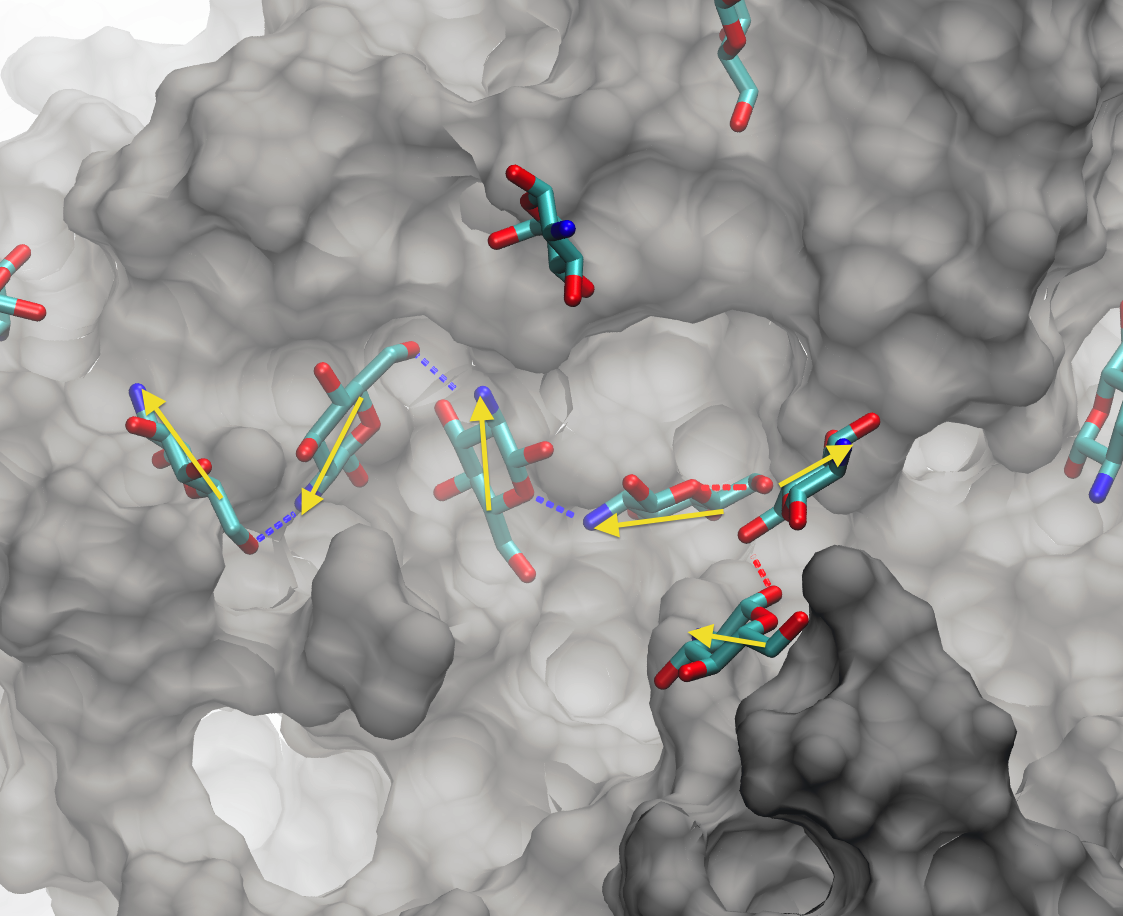
\includegraphics[width=6in]{figures/results4/glucosamine_binding_direction_suggestive.png}
\caption[Polymer directionality]{A bound linear hydrogen-bonded chain of glucosamine in the putative carbohydrate-binding groove of the C-terminal domain.  The yellow arrows are drawn as a guide for the directionality of the chain.}
\label{fig:directionality}
\end{figure}

% I don't fully understand the directionality business.  Here is a hack job at summarizing what it is from readings.
% From wikipedia -- An oligosaccharide has both a reducing and a non-reducing end. The reducing end of an oligosaccharide is the monosaccharide residue with hemiacetal functionality, thereby capable of reducing the Tollens’ reagent, while the non-reducing end is the monosaccharide residue in acetal form, thus incapable of reducing the Tollens’ reagent.[2] The reducing and non-reducing ends of an oligosaccharide are conventionally drawn with the reducing-end monosaccharide residue furthest to the right and the non-reducing (or terminal) end furthest to the left.[2]

% directionality paper
% http://www.jbc.org/content/274/37/26557.full


%%%%%%%%%%%%%%%%%%%%%% Future work %%%%%%%%%%%%%%%%%%%%%%
% What is the name for positively charged glucosamine molecules? Is there a 3-letter abbrev. for it?
% This paragraph can be part of the discussion.
As part of future work, it may be interesting to employ a similar approach to investigate the binding of glucosamine (GlcNH$_3^+$) monosaccharides and polysaccharides to PgaB.  Various analyses (eg. time evolution of RMSD, RMSF of the protein, principle component analysis, etc.) can be done to quantify protein dynamics, especially the mobility of the two domains. Furthermore, it will be interesting to investigate how dynamics may be correlated to the function of PgaB.  Finally, it will be interesting to predict GlcNac and GlcNH$_3^+$ binding modes and binding constants from MD simulations so that they can be compared with corresponding future experimental results.

\section{Acknowledgements}
This work was done in collaboration with Dustin Little, Dr. Lynne Howell and Dr. Mark Nitz.

\begin{figure}[htbp]
\centering
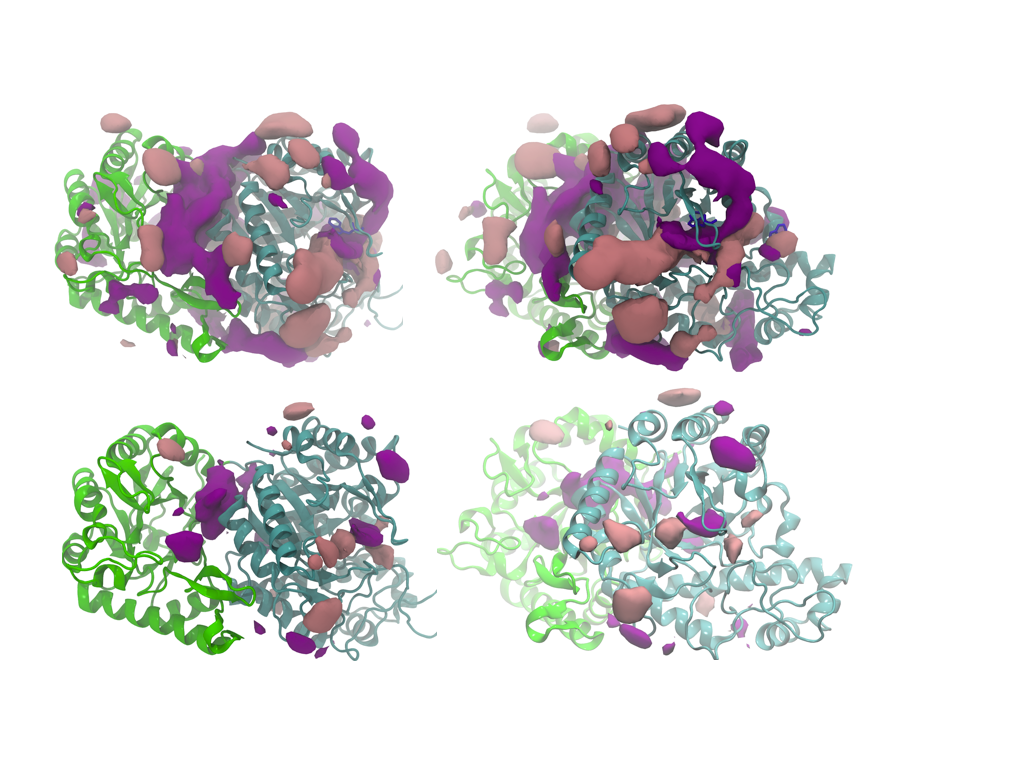
\includegraphics[width=7in]{figures/results4/pnag_nag_sdf_zoomedout.png}
\caption{Comparisons of the distributions of bound PNAG and NAG.}
\label{fig:pnag_nag_overlapped_zoomedout}
\end{figure}

\begin{figure}[htbp]
\centering
\includegraphics[width=7in]{figures/results4/salt_distribution.png}
\caption[Ionic distribution]{\textbf{Not yet rendered}. Spatial probability distribution of salt ions around \pgab}
\label{fig:salt_density_distribution}
\end{figure}

\begin{figure}[htbp]
\centering
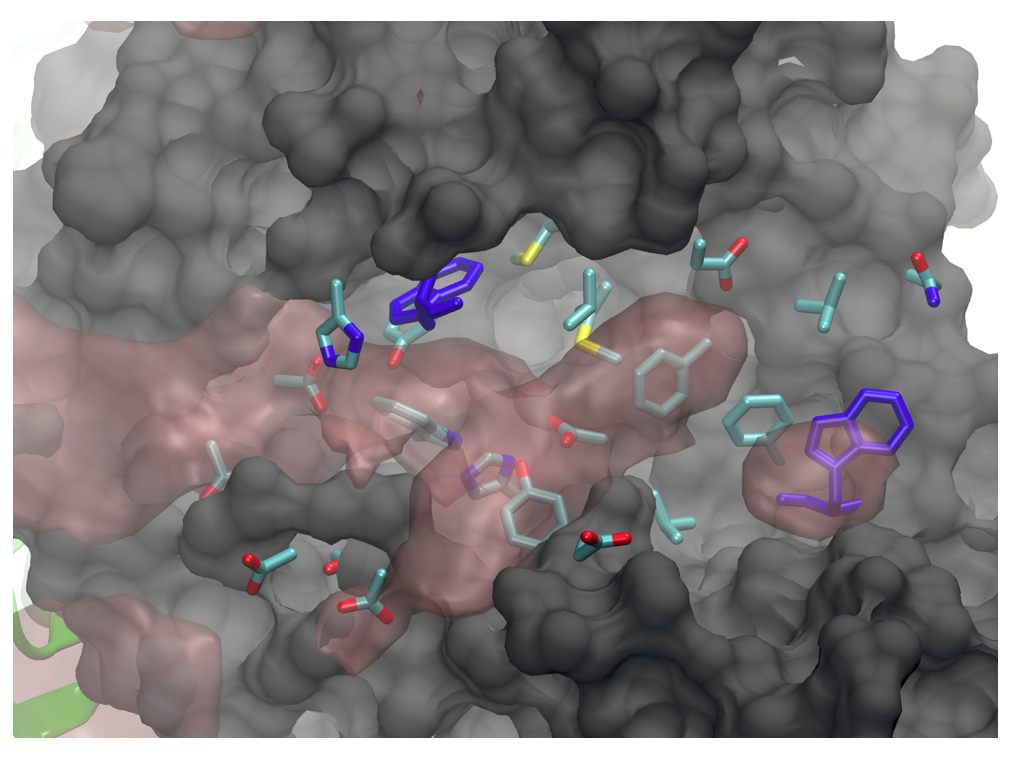
\includegraphics[width=6.23in]{figures/results4/nag_cterminal_zoomedin.png}
\caption{Distribution of NAG in the binding groove in the C-terminal domain.}
\label{fig:nag_cterminal_zoomedin}
\end{figure}


\begin{singlespace}
\addcontentsline{toc}{section}{Bibliography}
\bibliographystyle{elsart-num}
\bibliography{/Users/grace/github/thesis/document/results4/results4}
\end{singlespace}

% Objective of this work: 
% Binding surface - Map out a binding surface for both domains - We don't know what the C-Terminal domain is responsible for.  
% Compare and predict binding affinities.  Dustin is trying to get experimental data and co-crystal structures.

% Dustin -- But to get back to your main idea - i'm blabbering on here, other then the density map and binding constants. I guess it would be nice to see where the most flexible parts of the protein are - and what this might correlate too. What other quantitative values can you obtain?

% protein motion -- dynamics of the protein - can it be related to how it might function?
% \begin{itemize}
% 	\item Rmsd vs. time for the entire protein
% 	\item Rmsd vs. time for each of the individual domains
% 	\item Rmsf of the protein
% \end{itemize}

% % FIGURE
% \begin{figure}[pgab_rmsd]
% \centering
% 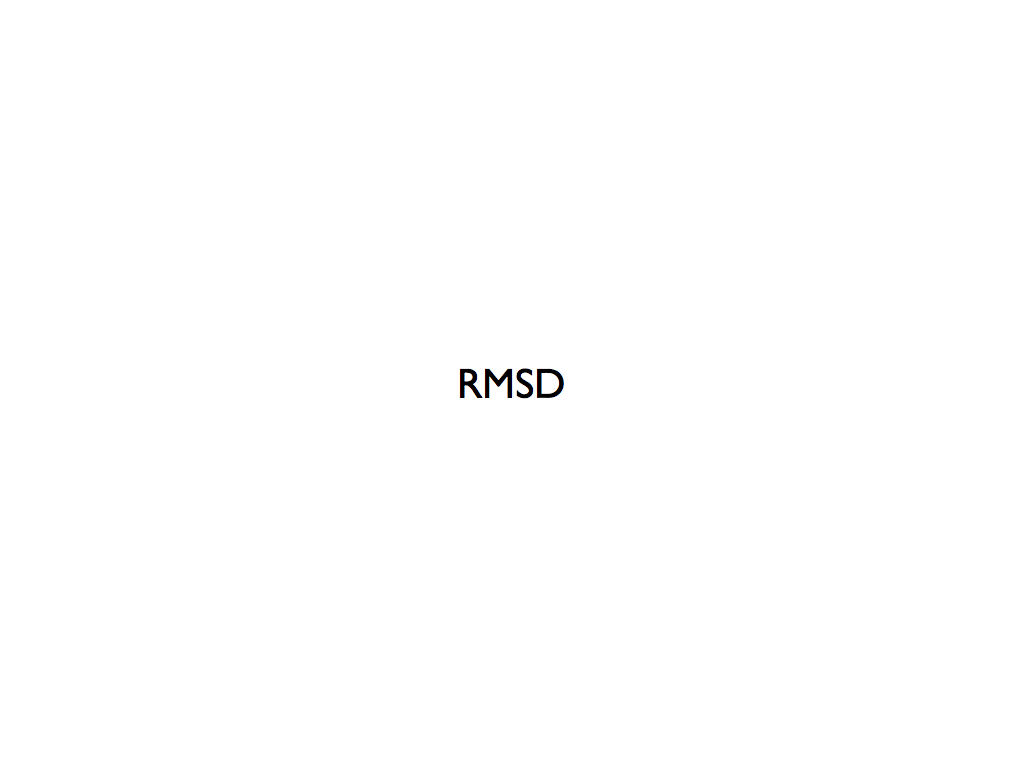
\includegraphics[height=4.1in, width=6.23in]{figures/pgab_rmsd.jpg}
% \caption[PgaB protein dynamics]{Time evolution of RMSD of PgaB from its crystal state}
% \label{fig:pgab_rmsd}
% \end{figure}
% 
% % FIGURE
% \begin{figure}[pgab_rmsf]
% \centering
% 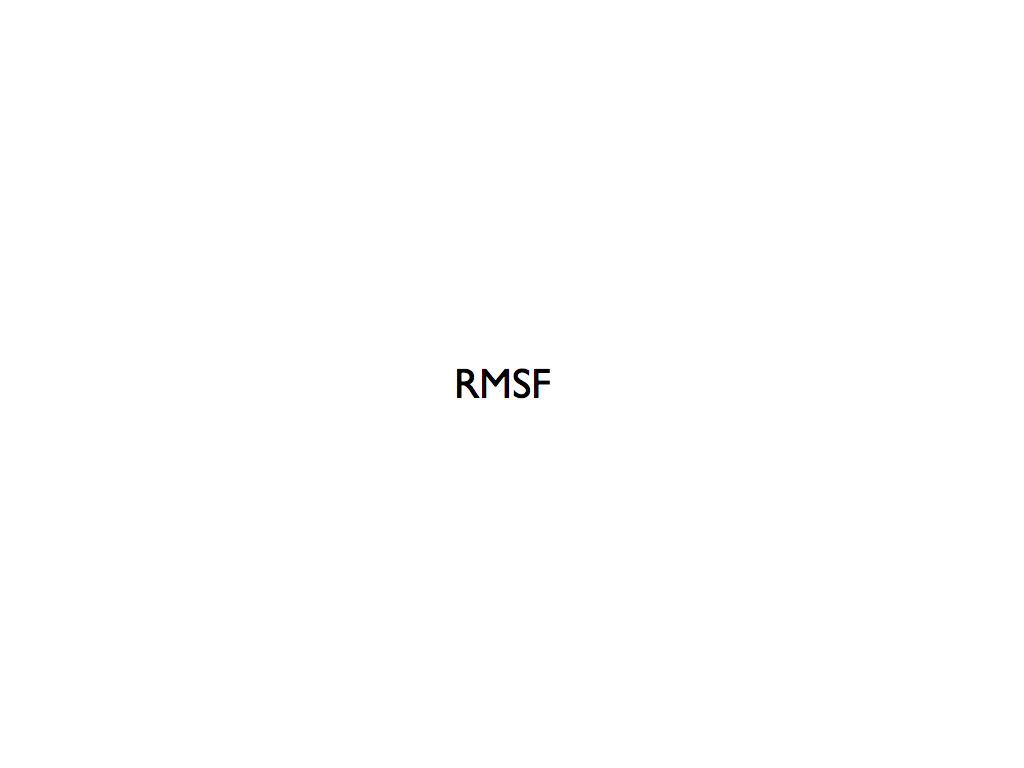
\includegraphics[height=4.1in, width=6.23in]{figures/pgab_rmsf.jpg}
% \caption[PgaB protein dynamics]{Time evolution of RMSD of PgaB from its crystal state}
% \label{fig:pgab_rmsf}
% \end{figure}

% FIGURE
% \begin{figure}[pgab_domains]
% \centering
% 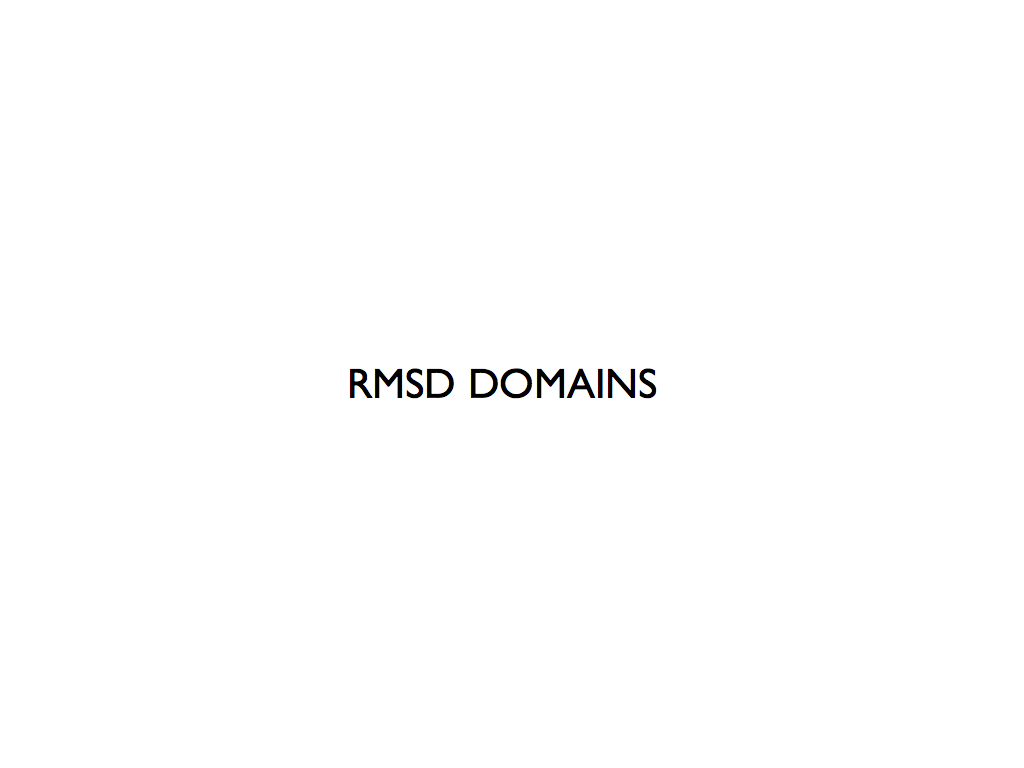
\includegraphics[height=4.1in, width=6.23in]{figures/pgab_domains.jpg}
% \caption[PgaB protein dynamics]{Time evolution of RMSD of PgaB from its crystal state}
% \label{fig:pgab_domains}
% \end{figure}